\section{Instruction Fetch}
The purpose of this unit is to:
\begin{itemize}
	\item hold the current value of the program counter (\texttt{PC}); 
	\item increment it when executing sequential code;
	\item fetch the next instruction from instruction memory
\end{itemize}

\subsection{Structure} A RTL description would contain a \texttt{PC} register, treated as a special register within the processor and an incrementer to compute \texttt{PC+4}. Normally, the PC is updated with the next sequential address. However, when a jump occurs, a selection logic driven by the control unit inside the ID stage causes the PC to be updated using an address coming from a dedicated adder that computes the target address for jumps or branches. In the case of a stall, the PC is not updated at all and the same instruction is refetched from memory.

This stage reads from the instruction memory, requiring a 32-bit output port to deliver the desired address and a 32-bit input port to receive the instruction word. 
\begin{figure}
	\centering
	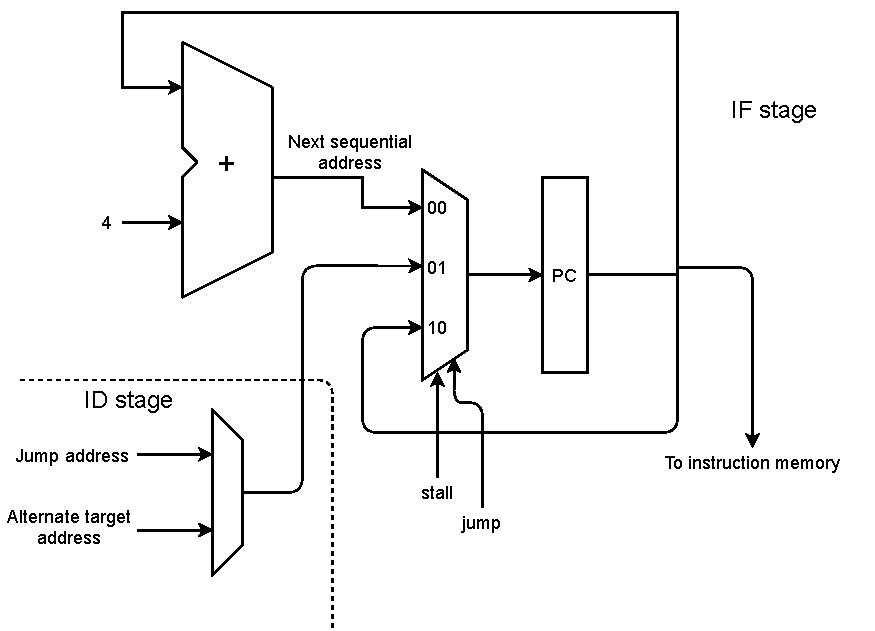
\includegraphics[width=0.6\textwidth]{../images/IF.pdf}
	\caption{RTL schematic of the instruction fetch stage, with part of the ID stage reported which selects the right jump address according to whether it is triggered by a jump instruction or a misprediction.}
\end{figure}